% Options for packages loaded elsewhere
\PassOptionsToPackage{unicode}{hyperref}
\PassOptionsToPackage{hyphens}{url}
%
\documentclass[
  ignorenonframetext,
]{beamer}
\usepackage{pgfpages}
\setbeamertemplate{caption}[numbered]
\setbeamertemplate{caption label separator}{: }
\setbeamercolor{caption name}{fg=normal text.fg}
\beamertemplatenavigationsymbolsempty
% Prevent slide breaks in the middle of a paragraph
\widowpenalties 1 10000
\raggedbottom
\setbeamertemplate{part page}{
  \centering
  \begin{beamercolorbox}[sep=16pt,center]{part title}
    \usebeamerfont{part title}\insertpart\par
  \end{beamercolorbox}
}
\setbeamertemplate{section page}{
  \centering
  \begin{beamercolorbox}[sep=12pt,center]{part title}
    \usebeamerfont{section title}\insertsection\par
  \end{beamercolorbox}
}
\setbeamertemplate{subsection page}{
  \centering
  \begin{beamercolorbox}[sep=8pt,center]{part title}
    \usebeamerfont{subsection title}\insertsubsection\par
  \end{beamercolorbox}
}
\AtBeginPart{
  \frame{\partpage}
}
\AtBeginSection{
  \ifbibliography
  \else
    \frame{\sectionpage}
  \fi
}
\AtBeginSubsection{
  \frame{\subsectionpage}
}
\usepackage{amsmath,amssymb}
\usepackage{lmodern}
\usepackage{ifxetex,ifluatex}
\ifnum 0\ifxetex 1\fi\ifluatex 1\fi=0 % if pdftex
  \usepackage[T1]{fontenc}
  \usepackage[utf8]{inputenc}
  \usepackage{textcomp} % provide euro and other symbols
\else % if luatex or xetex
  \usepackage{unicode-math}
  \defaultfontfeatures{Scale=MatchLowercase}
  \defaultfontfeatures[\rmfamily]{Ligatures=TeX,Scale=1}
\fi
% Use upquote if available, for straight quotes in verbatim environments
\IfFileExists{upquote.sty}{\usepackage{upquote}}{}
\IfFileExists{microtype.sty}{% use microtype if available
  \usepackage[]{microtype}
  \UseMicrotypeSet[protrusion]{basicmath} % disable protrusion for tt fonts
}{}
\makeatletter
\@ifundefined{KOMAClassName}{% if non-KOMA class
  \IfFileExists{parskip.sty}{%
    \usepackage{parskip}
  }{% else
    \setlength{\parindent}{0pt}
    \setlength{\parskip}{6pt plus 2pt minus 1pt}}
}{% if KOMA class
  \KOMAoptions{parskip=half}}
\makeatother
\usepackage{xcolor}
\IfFileExists{xurl.sty}{\usepackage{xurl}}{} % add URL line breaks if available
\IfFileExists{bookmark.sty}{\usepackage{bookmark}}{\usepackage{hyperref}}
\hypersetup{
  pdftitle={YOUR PAPER TITLE},
  pdfauthor={YOUR NAME},
  hidelinks,
  pdfcreator={LaTeX via pandoc}}
\urlstyle{same} % disable monospaced font for URLs
\newif\ifbibliography
\setlength{\emergencystretch}{3em} % prevent overfull lines
\providecommand{\tightlist}{%
  \setlength{\itemsep}{0pt}\setlength{\parskip}{0pt}}
\setcounter{secnumdepth}{-\maxdimen} % remove section numbering
\usepackage{booktabs}
\ifluatex
  \usepackage{selnolig}  % disable illegal ligatures
\fi

\title{YOUR PAPER TITLE}
\author{YOUR NAME}
\date{Social Media and Web Analytics, 2021}

\begin{document}
\frame{\titlepage}

\begin{frame}{Motivation}
\protect\hypertarget{motivation}{}
\textbf{One slide, motivating your project}

\textbf{Video Recording of your presentation must be less than 6 minutes
long!}

\begin{itemize}
\tightlist
\item
  Bullets
\item
  Bullets
\end{itemize}

\begin{enumerate}
\tightlist
\item
  Numbered List
\item
  Numbered List
\end{enumerate}
\end{frame}

\begin{frame}{Data}
\protect\hypertarget{data}{}
\textbf{One slide explaining the data}

\begin{center}\includegraphics[width=0.45\linewidth]{../output/SummaryTable} \end{center}
\end{frame}

\begin{frame}{Methodology}
\protect\hypertarget{methodology}{}
\textbf{One slide explaining your methods}

Here's an equation\ldots{}

\[
y_i = x_i \beta + \varepsilon_i
\]
\end{frame}

\begin{frame}{Results}
\protect\hypertarget{results}{}
\textbf{One slide showing your main result}

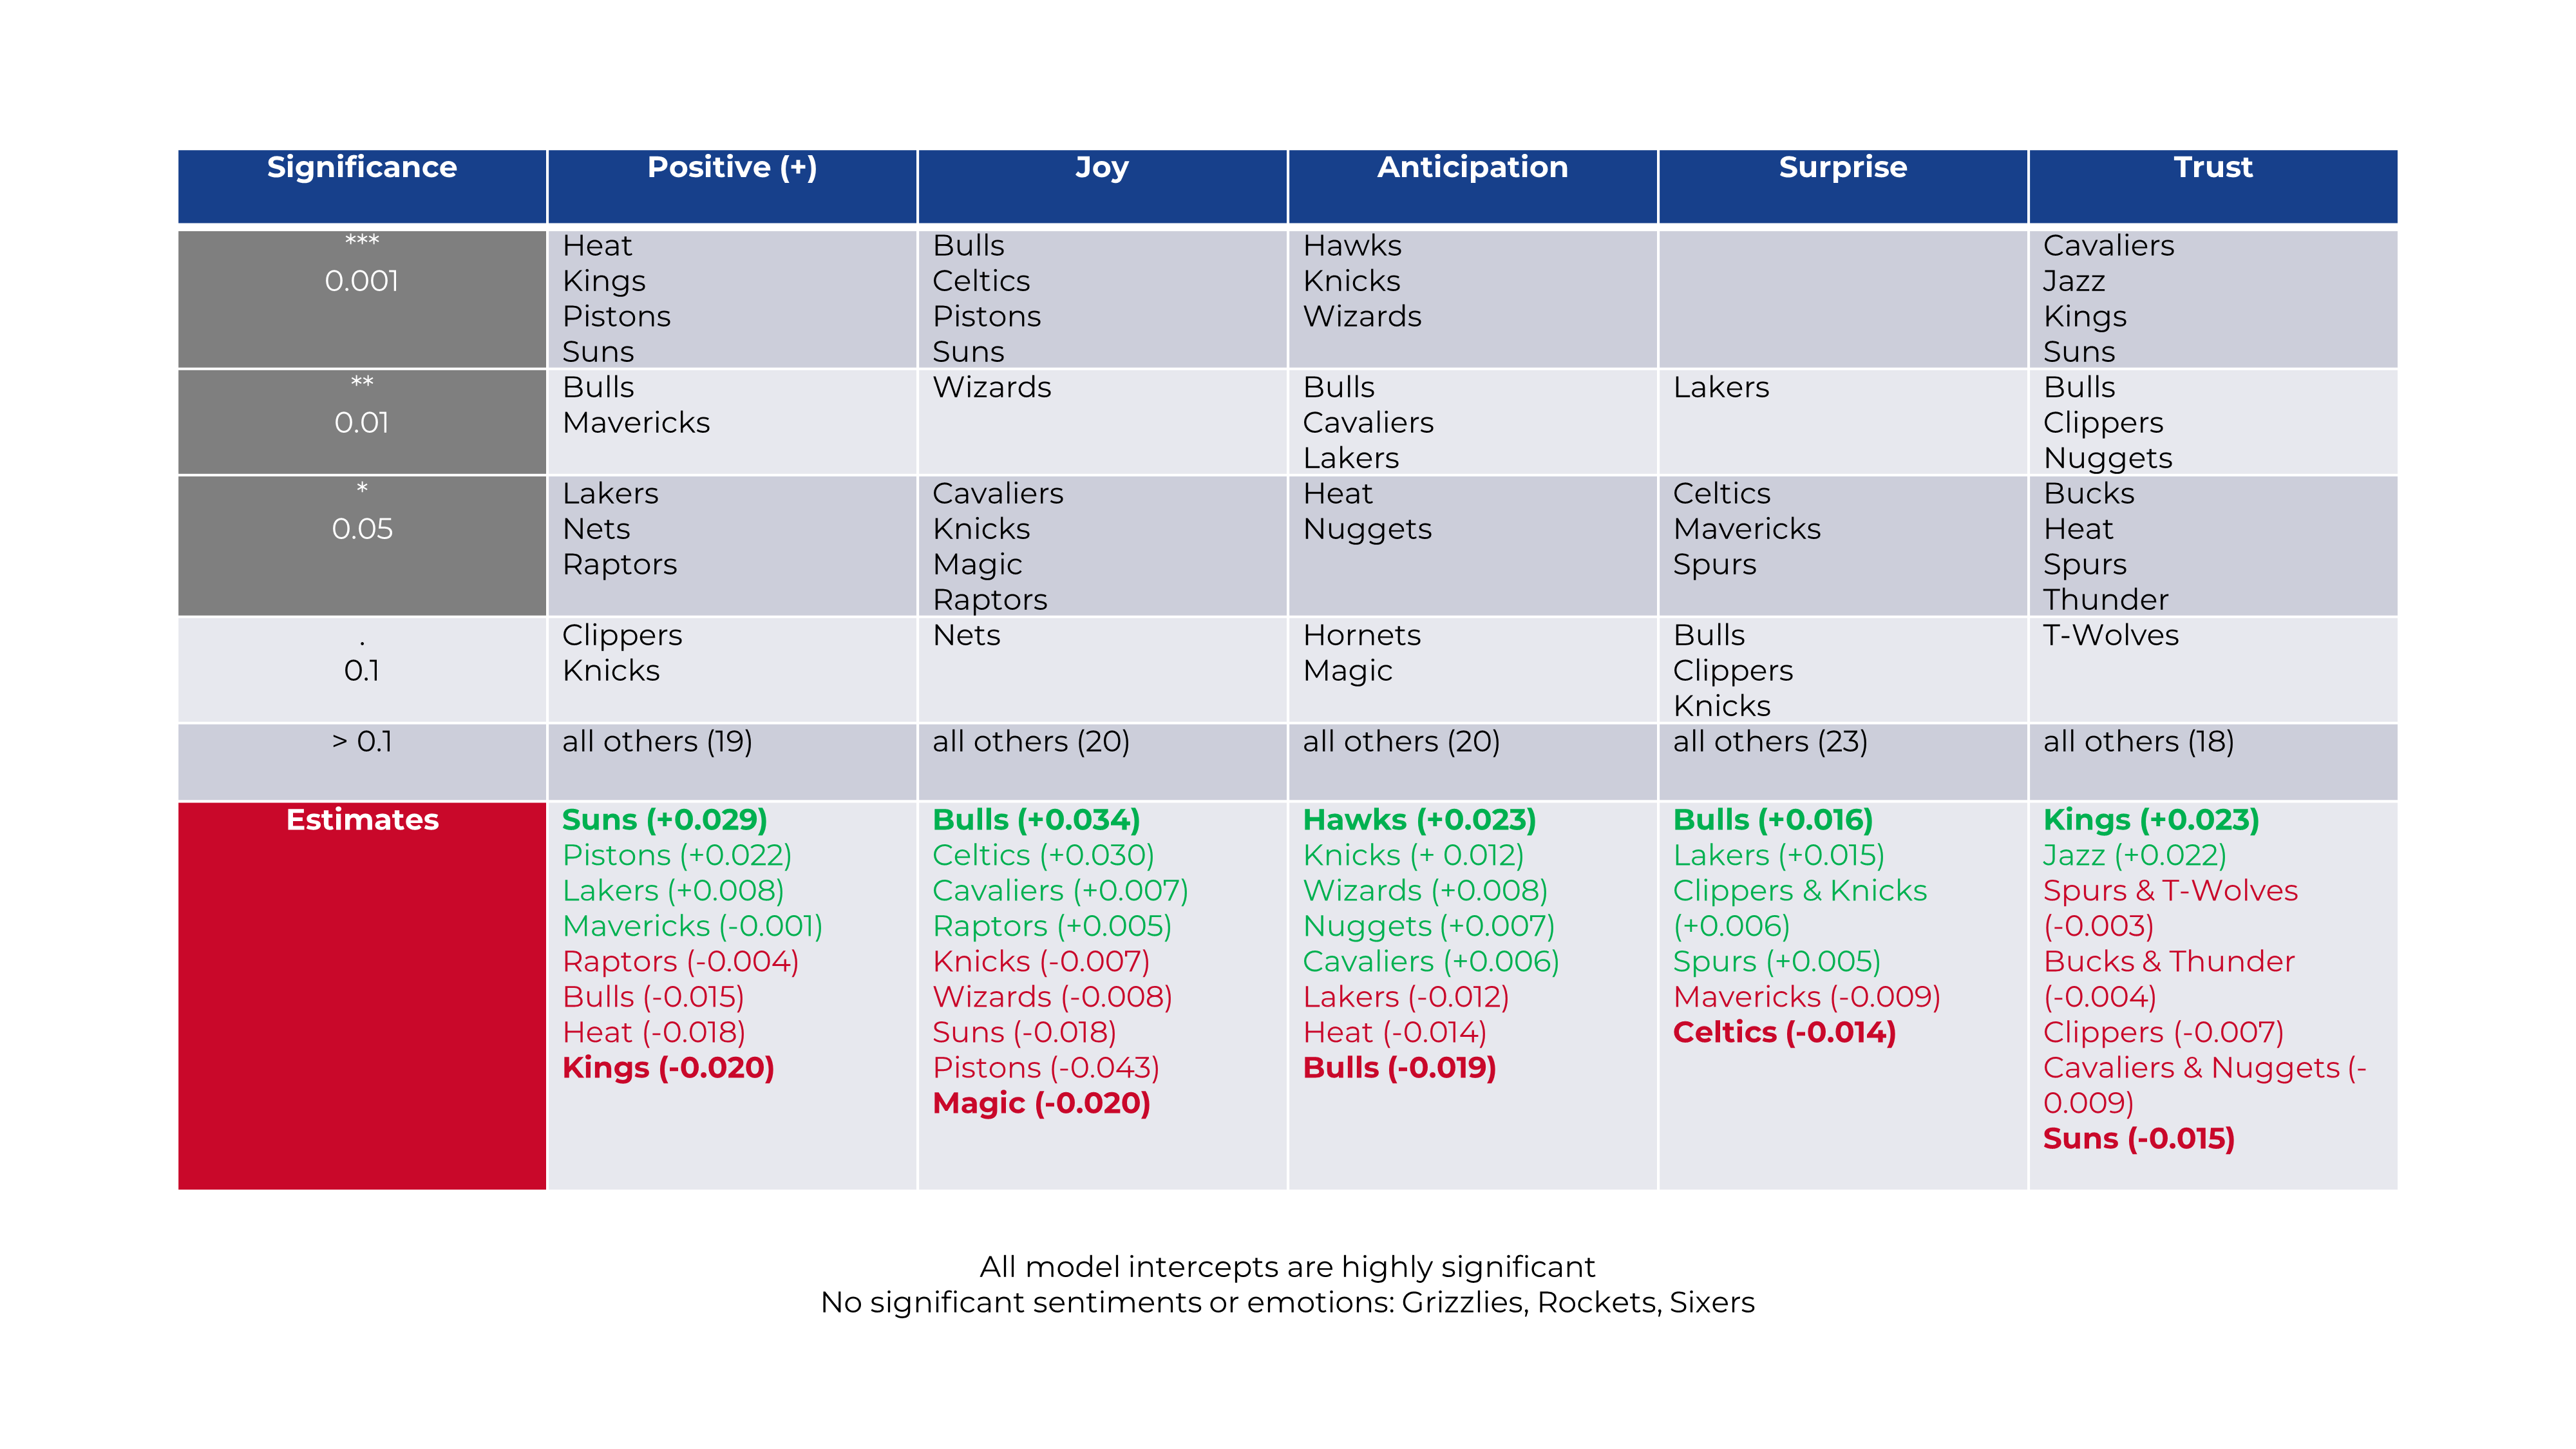
\includegraphics[width=55.56in]{../output/Positive Sentiments & Emotions}
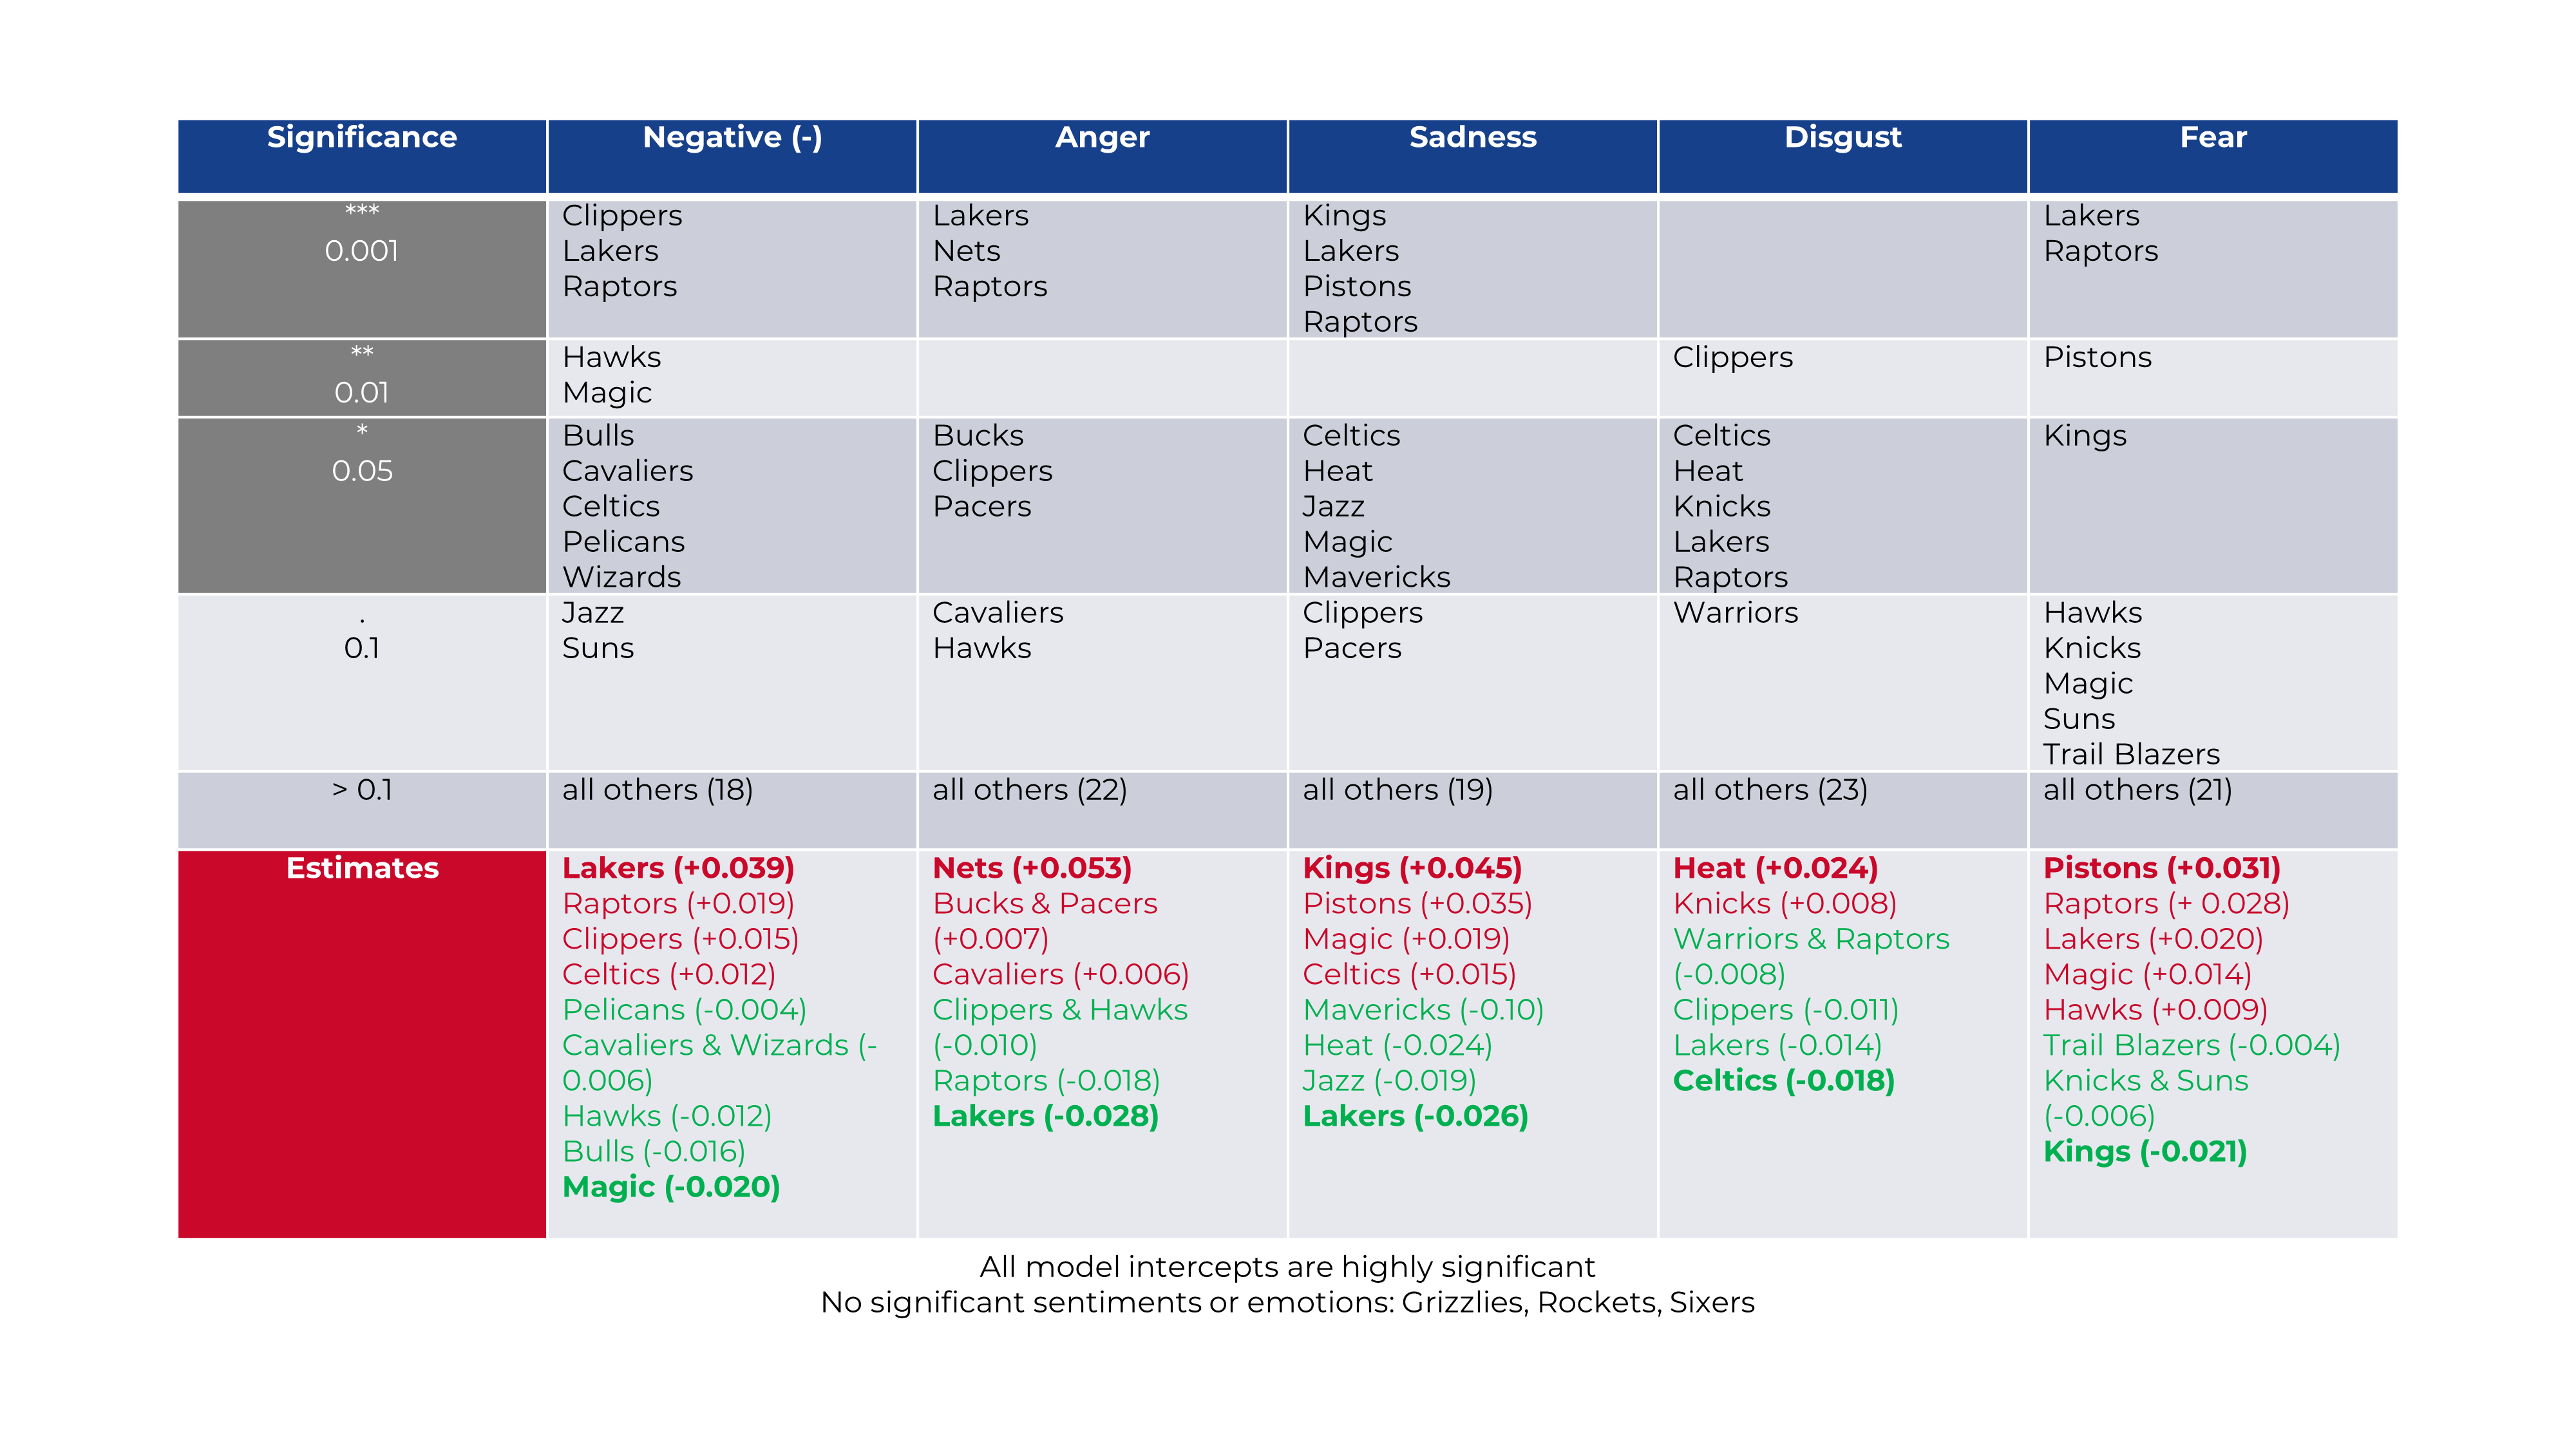
\includegraphics[width=55.56in]{../output/Negative Sentiments & Emotions}
\end{frame}

\begin{frame}{Conclusion}
\protect\hypertarget{conclusion}{}
\textbf{One slide with your concluding remarks} The analysis revealed
that the sentiments and emotions towards different NBA teams are not
only different, but also ambivalent in its direction. There are no teams
that are ``purely'' perceived in a negative or positive manner. This
observation is accurate for every team except for the three franchises
that didn't induce any significant Exemplary for this, the LA Lakers are
the most ``hated'' franchise in this sample, yet they are also unlikely
to be perceived in combination with angry or sad feelings. Recent
success seems to be an important factor how teams are perceived on
Twitter. Given this implication, marketers should exploit recent success
in the league with their marketing campaigns to exploit this - for
example after a big playoff win.
\end{frame}

\end{document}
